\subsection{Experimental Methodology and Results}
In the following paragraphs, we report the results of our experiments.

\subsubsection{RQ1. Mono-objective SBSE Validation}
\paragraph{Method}
In this experiment, we generate a set of random Csmith programs \textit{"the training set"} and apply different mono-objective algorithms to evaluate the non-functional properties of produced binaries. We compare as well manually generated sequences to standard GCC optimization levels. Our quality metric in this experiment is the percentage of overall performance improvement across all programs under test compared to a non-optimized version. The goal of this initial experiment is to: (1) evaluate the effectiveness of our component-based infrastructure to extract non-functional properties such as memory and CPU consumptions; (2) evaluate the performance of our proposed diversity-based exploration of optimization sequences (NS) to GA and RS; and finally (3) find the optimal solution relative to the input training set.




To answer the first research question RQ1, we implement three mono-objective algorithms GA and RS as well our NS adaptation for optimization sequences generation. As it is shown on the left side of figure 3, we used NOTICE to search for best optimization sequence from a set of input programs. For this reason, we generated 10 random programs using Csmith \textit{"training set"} and apply the generated sequences to these programs. Thus, the code quality objective function in this
experiments is equal to the average individual performance fitness values for all programs under test. The non-functional property could be CR, MR or S. It depends on the user design choice.
\paragraph{Results}
The goal of thus experiement is to 
\begin{table}[h]
	\centering
	\caption{My caption}
	\label{my-label}
	\begin{tabular}{|l|l|l|l|l|l|l|c|}
		\hline
		& O1                    & O2                    & O3                    & Ofast                 & RS                    & GA                    & NS \\ \hline
		S  & \multicolumn{1}{c|}{} & \multicolumn{1}{c|}{} & \multicolumn{1}{c|}{} & \multicolumn{1}{c|}{} & \multicolumn{1}{c|}{} & \multicolumn{1}{c|}{} &    \\ \hline
		MR &                       &                       &                       &                       &                       &                       &    \\ \hline
		CR &                       &                       &                       &                       &                       &                       &    \\ \hline
	\end{tabular}
\end{table}
\subsubsection{RQ2. Sensitivity}
\paragraph{Method}
Another interesting experiment is to test the sensitivity of training set programs to best optimal sequence previously discovered in RQ1. To do so, we apply best discovered optimizations to new unseen Csmith and CBench programs and compared the performance results. The idea of this experiment is to test whether only Csmith programs are more sensitive to compiler optimizations or not. If so, this will be useful for compiler users and researchers to use NOTICE in order to build general optimization sequences from their representative training set programs.



To test the generality of the best optimizations discovered, we apply in RQ2 these sequences to new unseen programs as it is shown on the right part of figure 3. We choose to apply optimizations to new 10 Csmith and 10 Cbench programs. Through this experiment, we would like to test the sensitivity of input programs and general applicability of optimization sequences.
\paragraph{Results}
\subsubsection{RQ3. Impact of optimizations on resource consumption}
\paragraph{Method}
To answer this question, we use NOTICE to generate best sequences per-Benchmark in term of speedup, and compare the memory footprint and CPU consumption of best optimized code. The goal of this experiment is to provide an understanding of the resource consumption of generated code by GCC. 




To answer RQ3, we study the impact of these optimizations on memory and CPU consumption using our Docker-based infrastructure. Following again a mono-objective approach, we try in this experiment to maximize the speedup \textit{S} and study in the mean time the impact of \textit{S} on resource consumptions namely memory and CPU usage. In this experiment, we choose 5 Cbench programs to investigate resource consumptions per-benchmark.
\paragraph{Results}
\begin{figure}[h]
	\centering
	\includegraphics[width=1.\linewidth]{Ressources/infra_novelty_stat2.png}
	\caption{Evaluating the speedup after applying standard optimization options compared to best generated optimization using NS}
\end{figure}
\subsubsection{RQ4. Trade-offs between non-functional properties}
\paragraph{Method}
A multi-objective approach provides a trade-off between two objectives where the developers can select their desired solution from the Pareto-optimal front. The goal of this experiment is to put more emphasis on resource consumption and use multi-objective algorithms to find trade-offs between non-functional properties of generated code like $<$ExecutionTime--MemoryUsage$>$, etc.



Finally in RQ4, we try to use NOTICE to find trade-offs between non-functional properties. In this experiment, we choose to focus on the trade-off $<$ExecutionTime--MemoryUsage$>$. We report the comparison results of three multi-objective algorithm adaptations NSGA-II, RS and NS. 
Sequences evaluation is done across 5 Cbench programs as it is conducted in RQ1.
We evaluate the quality of the obtained Pareto optimal optimization levels, both qualitatively by visual inspection of the Pareto frontiers, and quantitatively by using the HV metric.
\paragraph{Results}
In this section, we compare our NS adaptation for optimizations generation to the current, state-of-the-art multi-objective approaches namely NSGA-II and RS. Two tradeoffs are investigated in this section; $<$execution time--memory usage$>$ and $<$execution time--CPU usage$>$.

First, we conduct a quantitative study by comparing the HV metric for both tradeoffs than we conduct a quantitative study through pareto front distribution charts.
\subsection{Discussions}
\subsection{Discussions}










\begin{figure}[!t]
	\centering
	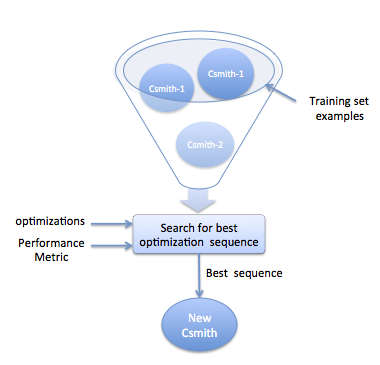
\includegraphics[width=1\hsize]{Ressources/approach by example.png}
	\caption{fig}
\end{figure}

\begin{figure}[!t]
	\centering
	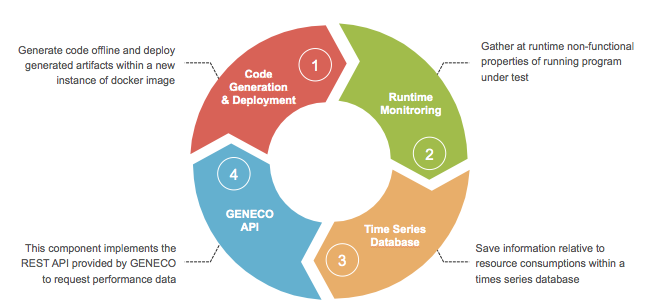
\includegraphics[width=1\hsize]{Ressources/geneco approach.png}
	\caption{fig}
\end{figure}

\begin{figure}[!t]
	\centering
	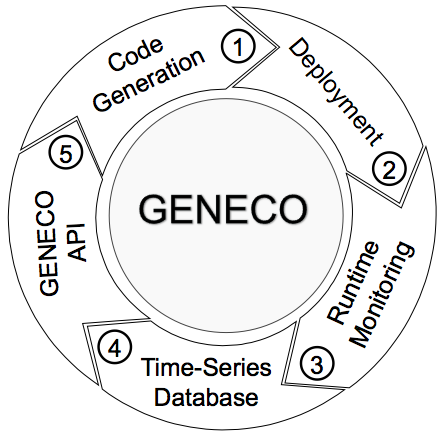
\includegraphics[width=1\hsize]{Ressources/genecoApproach22.png}
	\caption{fig}
\end{figure}
\iffalse
\begin{table}[]
	\centering
	\caption{My caption}
	\label{my-label}
	\begin{tabular}{@{}|l|c|c|c|c|c|c|c|c|c|c|c|c|c|c|c|c|c|c|c|c|@{}}
		\toprule
		\multirow{2}{*}{} & \multicolumn{2}{c|}{CB1} & \multicolumn{2}{c|}{CB2} & \multicolumn{2}{c|}{CB3} & \multicolumn{2}{c|}{CB4} & \multicolumn{2}{c|}{CB5} & \multicolumn{2}{c|}{CS1} & \multicolumn{2}{c|}{CS2} & \multicolumn{2}{c|}{CS3} & \multicolumn{2}{c|}{CS4} & \multicolumn{2}{c|}{CS5} \\ \cmidrule(l){2-21} 
		& Ox & Best & Ox & Best & Ox & Best & Ox & Best & Ox & Best & Ox & Best & Ox & Best & Ox & Best & Ox & Best & Ox & Best \\ \midrule
		Execution Speedup & \begin{tabular}[c]{@{}c@{}}4\%\\ (O3)\end{tabular} &  &  &  &  &  &  &  &  &  &  &  &  &  &  &  &  &  &  &  \\ \midrule
		Memory & \begin{tabular}[c]{@{}c@{}}4\%\\ (O3)\end{tabular} &  &  &  &  &  &  &  &  &  &  &  &  &  &  &  &  &  &  &  \\ \midrule
		CPU & \begin{tabular}[c]{@{}c@{}}4\%\\ (O3)\end{tabular} &  &  &  &  &  &  &  &  &  &  &  &  &  &  &  &  &  &  &  \\ \midrule
		Compilation Speedup &  &  &  &  &  &  &  &  &  &  &  &  &  &  &  &  &  &  &  &  \\ \midrule
		Code Size &  &  &  &  &  &  &  &  &  &  &  &  &  &  &  &  &  &  &  &  \\ \bottomrule
	\end{tabular}
\end{table}
\fi


\begin{figure}[h]
	\centering
	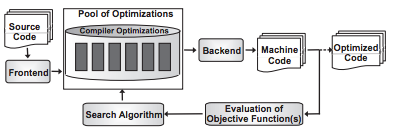
\includegraphics[width=1\hsize]{Ressources/compilation.png}
	\caption{fig}
\end{figure}
\begin{figure}[h]
	\centering
	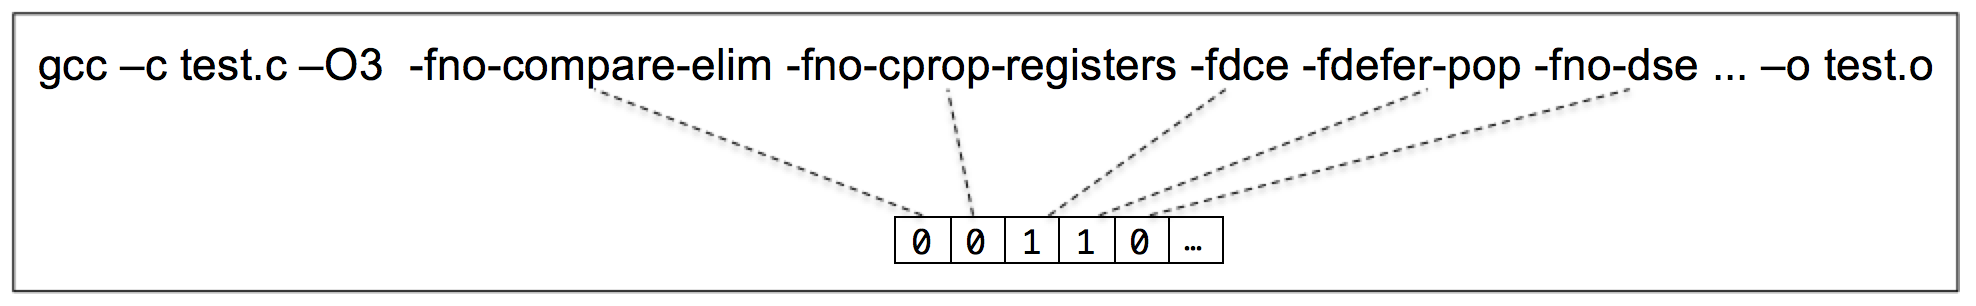
\includegraphics[width=1\hsize]{Ressources/individual.png}
	\caption{fig}
\end{figure}

